% The solubility parity float.  \input this where the arm comparison is discussed
% (it belongs beside Fig.~\ref{fig:paradox}, which reports the same arms as bars).
%
% figure*, width=\linewidth: the canvas is drawn at \textwidth (504.47 pt) and the tight
% bbox crops it to 486.6 pt, so at \linewidth it is ENLARGED by 1.037x and every type size
% in it prints at or above the size it was set at.  Setting it in one column instead would
% halve that and put the mathtext subscripts under 4 pt.  Do not add a width fraction.
%
% THE CAPTION IS A DESCRIPTION OF WHAT IS DRAWN and nothing else (supervisor, 2026-08-09).
% It was 194 words over 13 printed lines, taller on the page than the plot; three of its
% sentences reconciled the panels' seed-42 statistics against the three-seed bars of
% Fig.~\ref{fig:paradox}, and one explained why the axes were mostly empty.  The figure now
% prints its own seed, and the axes are set to the measurement, so neither is a caption's
% job.  Do not restore an argument here: the panel-vs-bar difference is a fact
% tab:si-arms already carries, per seed and per arm.
%
% NOT fig:parity.  That label is the activity-coefficient parity on the n=60
% VT-2005-matched pairs, in the Supporting Information.  Two different figures.
%
% Regenerate:
%   KMP_DUPLICATE_LIB_OK=TRUE PYTHONPATH=src python scripts/analysis/make_parity_figure.py \
%       --e5-dir results/e5_sigma_grounding --seed 42 --out-dir paper/figs \
%       --dump-json paper/figs/fig_parity_lnx2.numbers.json
% Every number the caption quotes from the panels is in that .numbers.json.
\begin{figure*}[t]
\centering
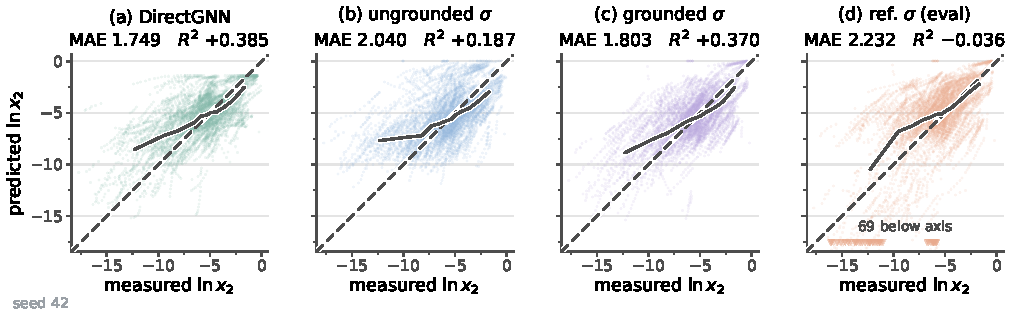
\includegraphics[width=\linewidth]{figs/fig_parity_lnx2.pdf}
\caption{Solubility parity for four arms of the controlled comparison: predicted against
measured $\lnx$ on the $5608$ labelled test rows of the scaffold split, which are $763$
solute--solvent pairs over $147$ solutes and $70$ solvents measured between $248$ and
$368$\,K. (a) DirectGNN, the closure-free control; (b) COSMO-SAC over an unsupervised
$\sigma$-profile; (c) the same closure with $\sigma$-profile supervision during training;
(d) the arm of (c) with the reference VT-2005 profile substituted at evaluation. Dashed,
the identity. Solid, the median prediction in twelve equal-count bins of the measurement.
Each panel header carries that panel's own MAE and $R^2$. Both axes span the measured
range with a margin around it, and the markers along the foot of (d) are its $69$ predictions that fall
below the frame, each
at its own measured value. Panels (b), (c) and (d) come from the five-seed leak-free re-run: the
ungrounded, grounded and $\sigma$-oracle arms respectively.}
\label{fig:parity-lnx2}
\end{figure*}
